\documentclass[]{informeutn}

% Paquetes y configuraciones complementarias
\usepackage{csquotes}

\addbibresource{fuentes.bib}

% Unidades adicionales
\newcommand{\MHz}{\,\unit{\mega\hertz}}
\newcommand{\kB}{\,\unit{\kilo\byte}}

% Colores y estilos para listados de código
\definecolor{mygreen}{rgb}{0,0.6,0}
\definecolor{mygray}{rgb}{0.5,0.5,0.5}
\definecolor{mymauve}{rgb}{0.58,0,0.82}

\lstset{
  backgroundcolor=\color{white},
  basicstyle=\scriptsize\ttfamily,
  breakatwhitespace=false,
  breaklines=true,
  captionpos=b,
  commentstyle=\color{mygreen},
  extendedchars=true,
  literate={á}{{\'a}}1 {é}{{\'e}}1 {í}{{\'i}}1 {ó}{{\'o}}1 {ú}{{\'u}}1 {ñ}{{\~n}}1 {Á}{{\'A}}1 {É}{{\'E}}1 {Í}{{\'I}}1 {Ó}{{\'O}}1 {Ú}{{\'U}}1 {Ñ}{{\~N}}1,
  frame=single,
  keepspaces=true,
  keywordstyle=\color{blue},
  numbers=left,
  numbersep=5pt,
  numberstyle=\tiny\color{mygray},
  rulecolor=\color{black},
  showspaces=false,
  showstringspaces=false,
  showtabs=false,
  stepnumber=1,
  stringstyle=\color{mymauve},
  tabsize=4
}

% Metadatos del informe
\materia{Técnicas Digitales II}
\titulo{Trabajo Práctico N.º 4}
\subtitulo{Programación de la placa BluePill STM32F103 con FreeRTOS}
\comision{4R2}
\autores{Gastón Grasso 401892\\ Franco Palombo 401910\\ Angelo Prieto 401012}
\fecha{\today}

\begin{document}
  \maketitle
  \tableofcontents
  \setcounter{page}{1}
  \thispagestyle{plain}
  
  \chapter{Introducción}

En este trabajo práctico se aborda la integración y utilización de un sistema operativo en tiempo real
en sistemas embebidos basados en la arquitectura ARM Cortex-M3. A diferencia del paradigma secuencial tradicional
en bare-metal, el empleo de un kernel como FreeRTOS permite estructurar la aplicación en tareas concurrentes con
prioridades asignadas, garantizando determinismo temporal, modularidad y un uso predecible de los recursos del
microcontrolador.

\section{Objetivos del Trabajo Práctico}

El desarrollo se orienta a cumplir los siguientes objetivos específicos:

\begin{itemize}
  \item Configurar el núcleo de FreeRTOS para la arquitectura ARM Cortex-M3 presente en el microcontrolador
  STM32F103C8T6, ajustando los parámetros de temporización, gestión de memoria y planificación apropiativa.
  \item Diseñar e implementar tareas periódicas con diferentes niveles de prioridad, verificando el comportamiento
  del planificador apropiativo y evaluando la fracción de tiempo en reposo de la CPU mediante la función Idle Hook.
  \item Resolver un esquema clásico de productor-consumidor mediante mecanismos formales de comunicación y
  sincronización entre tareas provistos por el kernel: colas de mensajes y semáforos binarios.
  \item Integrar de forma segura la capa de interrupciones de periféricos de hardware con el entorno multitarea,
  utilizando las funciones especializadas de la API de FreeRTOS para rutinas de servicio de interrupción.
\end{itemize}


  \chapter{Ejercicio Práctico N.º 1: Tareas y Planificación}
\label{sec.ej1:planificacion}

\section{Descripción General}

El primer ejercicio tiene como propósito implementar un esquema de multitarea apropiativa
utilizando el núcleo de FreeRTOS, verificando la coexistencia de múltiples flujos de ejecución concurrentes con
diferentes niveles de prioridad y períodos de repetición.

El sistema debe ejecutar de forma simultánea tres actividades con restricciones temporales diferenciadas:
el parpadeo de un LED de señalización a frecuencia constante, la emisión periódica de una cadena de texto con datos
de diagnóstico a través del puerto serie USART1, y el cómputo de la disponibilidad de procesamiento mediante el monitoreo
de la tarea Idle.

\section{Estructura de Tareas y Prioridades}

Para satisfacer las consignas se definieron dos tareas de usuario explícitas y se habilitó la función \textit{IdleHook}
asociada a la tarea del sistema. En la tabla \ref{tab.ej1:tareas} se resumen los parámetros de configuración
asignados a cada tarea durante la inicialización.

\begin{table}[!ht]
\centering
\small
\caption{Parámetros de configuración de las tareas en el Ejercicio 1.}
\label{tab.ej1:tareas}
\begin{tabular}{llcccl}
\toprule
Tarea & Función & Prioridad & Stack & Período & Salida / Acción \\
\midrule
Tarea A & \texttt{vBlink} & 3 & 256 pal. & $\SI{100}{\milli\second}$ & Pin PC13 (LED) \\
Tarea B & \texttt{vSendTelemetry} & 2 & 256 pal. & $\SI{2000}{\milli\second}$ & USART1 (PA9) \\
Tarea C & \texttt{IdleHook} & 0 & Stack Idle & Continuo & Incremento de \texttt{ulIdleCount} \\
\bottomrule
\end{tabular}
\end{table}

La jerarquía de prioridades adoptada responde a los criterios fundamentales de los sistemas de tiempo real:

\begin{enumerate}
  \item \textbf{Tarea A (\texttt{vBlink}, prioridad 3)}: Se le asigna la prioridad más alta entre las tareas de usuario
    a fin de asegurar que el cambio de estado lógico en el pin PC13 no sufra fluctuaciones temporales inducidas
    por la actividad de comunicaciones serie. El período de conmutación se fijó en $\SI{100}{\milli\second}$, lo que
    determina un ciclo completo de encendido y apagado de $\SI{200}{\milli\second}$, cumpliendo con la frecuencia de
    parpadeo de $\SI{5}{\hertz}$.
  \item \textbf{Tarea B (\texttt{vSendTelemetry}, prioridad 2)}: Posee una prioridad intermedia. Se ejecuta una vez cada
    $\SI{2000}{\milli\second}$ ($\SI{2}{\second}$) para componer una cadena de texto en memoria y transmitirla byte a
    byte mediante el periférico USART1. Al disponer de menor prioridad que la Tarea A, si el temporizador de
    $\SI{100}{\milli\second}$ expira mientras la Tarea B está enviando datos, el planificador suspende su ejecución ,
    atiende el cambio de estado del LED y reanuda la transmisión serie.
  \item \textbf{Tarea C (\texttt{Idle Hook}, prioridad 0)}: La tarea de inactividad es instanciada internamente por
    FreeRTOS con la prioridad más baja del sistema. Ejecuta la función \texttt{vApplicationIdleHook()} únicamente cuando
    las tareas A y B se encuentran bloqueadas a la espera del vencimiento de sus respectivos intervalos de retardo.
\end{enumerate}

En la figura \ref{fig.ej1:cronograma} se ilustra el cronograma temporal del sistema y la dinámica de desalojo
conducida por el planificador del kernel.

\begin{figure}[!ht]
\centering
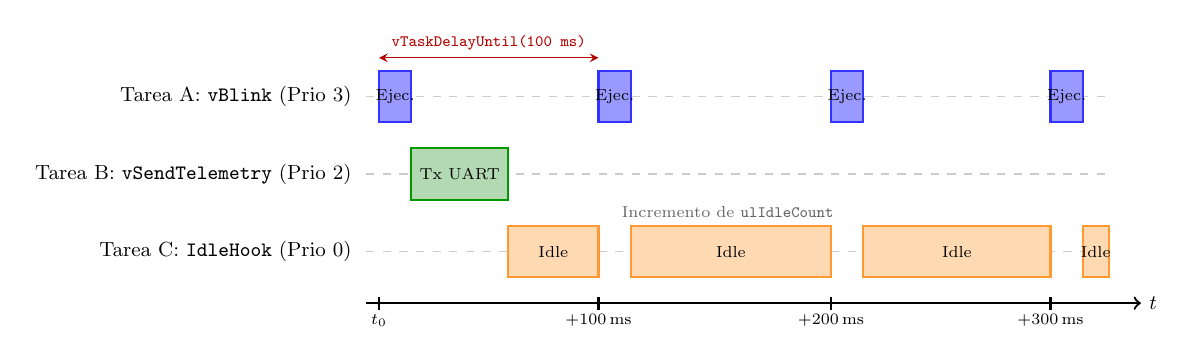
\begin{tikzpicture}[scale=0.82, transform shape, every node/.style={font=\small}]
  % Ejes de tareas
  \draw[->, thick] (0,0) -- (12,0) node[right] {$t$};
  \node[left] at (-0.1, 3.2) {Tarea A: \texttt{vBlink} (Prio 3)};
  \node[left] at (-0.1, 2.0) {Tarea B: \texttt{vSendTelemetry} (Prio 2)};
  \node[left] at (-0.1, 0.8) {Tarea C: \texttt{IdleHook} (Prio 0)};

  % Líneas base
  \draw[gray!40, dashed] (0, 3.2) -- (11.5, 3.2);
  \draw[gray!40, dashed] (0, 2.0) -- (11.5, 2.0);
  \draw[gray!40, dashed] (0, 0.8) -- (11.5, 0.8);

  % Tarea A (vBlink) - se ejecuta periódicamente cada 100 ms (pulsos breves)
  \fill[blue!40, draw=blue!80, thick] (0.2, 2.8) rectangle (0.7, 3.6) node[pos=0.5, black, font=\scriptsize] {Ejec.};
  \fill[blue!40, draw=blue!80, thick] (3.6, 2.8) rectangle (4.1, 3.6) node[pos=0.5, black, font=\scriptsize] {Ejec.};
  \fill[blue!40, draw=blue!80, thick] (7.2, 2.8) rectangle (7.7, 3.6) node[pos=0.5, black, font=\scriptsize] {Ejec.};
  \fill[blue!40, draw=blue!80, thick] (10.6, 2.8) rectangle (11.1, 3.6) node[pos=0.5, black, font=\scriptsize] {Ejec.};

  % Tarea B (vSendTelemetry) - ejecuta al inicio o cada 2 s, es desalojada o corre tras Tarea A
  \fill[green!50!black!30, draw=green!60!black, thick] (0.7, 1.6) rectangle (2.2, 2.4) 
    node[pos=0.5, black, font=\scriptsize] {Tx UART};

  % Tarea C (Idle Hook) - corre en todo el tiempo restante
  \fill[orange!30, draw=orange!80, thick] (2.2, 0.4) rectangle (3.6, 1.2) node[pos=0.5, black, font=\scriptsize] {Idle};
  \fill[orange!30, draw=orange!80, thick] (4.1, 0.4) rectangle (7.2, 1.2) node[pos=0.5, black, font=\scriptsize] {Idle};
  \fill[orange!30, draw=orange!80, thick] (7.7, 0.4) rectangle (10.6, 1.2) node[pos=0.5, black, font=\scriptsize] {Idle};
  \fill[orange!30, draw=orange!80, thick] (11.1, 0.4) rectangle (11.5, 1.2) node[pos=0.5, black, font=\scriptsize] {Idle};

  % Marcadores temporales
  \draw[thick] (0.2, -0.1) -- (0.2, 0.1) node[below=4pt, font=\scriptsize] {$t_0$};
  \draw[thick] (3.6, -0.1) -- (3.6, 0.1) node[below=4pt, font=\scriptsize] {$+100\,\mathrm{ms}$};
  \draw[thick] (7.2, -0.1) -- (7.2, 0.1) node[below=4pt, font=\scriptsize] {$+200\,\mathrm{ms}$};
  \draw[thick] (10.6, -0.1) -- (10.6, 0.1) node[below=4pt, font=\scriptsize] {$+300\,\mathrm{ms}$};

  % Flechas y anotaciones
  \draw[<->, >=stealth, red!70!black] (0.2, 3.8) -- (3.6, 3.8) 
    node[midway, above, font=\scriptsize] {\texttt{vTaskDelayUntil(100 ms)}};
  \node[above, font=\scriptsize, gray!80!black] at (5.6, 1.2) {Incremento de \texttt{ulIdleCount}};
\end{tikzpicture}

\caption{Cronograma de ejecución y asignación de CPU entre tareas en el Ejercicio 1.}
\label{fig.ej1:cronograma}
\end{figure}

\section{Recursos de FreeRTOS Utilizados}
\label{sec.ej1:recursos}

El funcionamiento del programa se apoya en los siguientes servicios y primitivas provistos por el kernel:

\subsection{Creación e Inicialización de Tareas}

\begin{lstlisting}[language=C]
res = xTaskCreate(vBlink, "Blink", 256, NULL, 3, NULL);
if (res != pdPASS) {
    while(1);
}
\end{lstlisting}

Se verifica sistemáticamente el valor de retorno. Si la función retorna un código distinto de \texttt{pdPASS}, se
detiene el flujo de ejecución en una condición segura de error.

Una vez configuradas las tareas y los periféricos de hardware mediante llamadas a registros CMSIS, la llamada a
\texttt{vTaskStartScheduler()} inicializa el temporizador SysTick a una cadencia de $\SI{1000}{\hertz}$
(\texttt{configTICK\_RATE\_HZ = 1000}) e inicia la ejecución de la tarea de mayor prioridad lista.

\subsection{Temporización Determinística con \texttt{vTaskDelayUntil}}

Para garantizar una periodicidad rigurosa sin acumulación de corrimiento temporal, se optó por el uso de
\texttt{vTaskDelayUntil()} en lugar de la función de retardo relativo convencional \texttt{vTaskDelay()}.

\begin{lstlisting}[language=C]
void vBlink(void *pvParameters) {
    TickType_t xLastTickEntry = xTaskGetTickCount();
    while (1) {
        GPIOC->ODR ^= GPIO_ODR_ODR13;
        vTaskDelayUntil(&xLastTickEntry, pdMS_TO_TICKS(100));
    }
}
\end{lstlisting}

La función toma como referencia el valor absoluto del conteo de ticks capturado al inicio (\texttt{xLastTickEntry})
y calcula internamente el instante exacto del siguiente desbloqueo sumando el número de ticks equivalente a
$\SI{100}{\milli\second}$ (\texttt{pdMS\_TO\_TICKS(100)}). De este modo, las fluctuaciones en el tiempo de
la ejecución del cuerpo del bucle no alteran el periodo global de repetición.

\subsection{Monitoreo de Carga con la Función Idle Hook}

En el archivo de configuración del kernel se estableció la directiva \texttt{configUSE\_IDLE\_HOOK = 1}. Bajo esta
condición, cada vez que la tarea Idle toma el procesador, invoca a la función de retorno definida por la aplicación:

\begin{lstlisting}[language=C]
void vApplicationIdleHook(void) {
    ulIdleCount++;
}
\end{lstlisting}

La variable \texttt{ulIdleCount} se declara como volátil (\texttt{volatile uint32\_t}) para evitar que el compilador
optimice su acceso en registros de CPU. En cada ciclo de telemetría ($\SI{2}{\second}$), la Tarea B formatea el valor
acumulado en dicha variable y lo transmite:

\begin{lstlisting}[language=C]
uint32_t length = sprintf(buffer, "%s%lu\r\n", string, ulIdleCount);
for (uint16_t i = 0; i < length; i++) {
    while ((USART1->SR & USART_SR_TXE) == 0);
    USART1->DR = buffer[i];
}
\end{lstlisting}

La velocidad de incremento de este contador permite corroborar que el microcontrolador permanece la mayor parte del
tiempo disponible en estado inactivo, dado que la Tarea A solo utiliza unos pocos microsegundos por ciclo para conmutar
el bit en el registro \texttt{GPIOC->ODR} y la Tarea B interviene únicamente una vez cada dos segundos.

  \chapter{Ejercicio Práctico N.º 2: Comunicación y Sincronización}
\label{sec.ej2:comunicacion}

\section{Descripción General}

El segundo ejercicio plantea la resolución del problema de productor-consumidor en un entorno con restricciones
temporales, integrando la adquisición de hardware mediante interrupciones con los mecanismos de sincronización
y pasaje de datos provistos por FreeRTOS.

El sistema debe adquirir de forma periódica una señal analógica conectada al canal 0 del convertidor analógico-digital
(pin PA0), transferir de manera segura la lectura hacia una tarea consumidora encargada de formatear y emitir el valor
digitalizado por el puerto serie USART1 cada $\SI{2000}{\milli\second}$, y mantener en paralelo la tarea de señalización
luminosa con el LED integrado en el pin PC13.

\section{Estructura de Tareas, Interrupciones y Prioridades}

La arquitectura del sistema divide las responsabilidades entre tres tareas independientes y una rutina de servicio
de interrupción (ISR) de hardware. En la tabla \ref{tab.ej2:tareas} se detallan sus atributos de ejecución.

\begin{table}[!ht]
\centering
\small
\caption{Atributos de tareas e interrupciones en el Ejercicio 2.}
\label{tab.ej2:tareas}
\begin{tabular}{llccl}
\toprule
Elemento & Tipo & Prioridad & Período & Función / Rol \\
\midrule
\texttt{vBlink} & Tarea & 3 & $\SI{100}{\milli\second}$ & Señalización en pin PC13 \\
\texttt{vReadADC} & Tarea & 2 & $\SI{100}{\milli\second}$ & Productor: disparo de ADC1 \\
\texttt{vSendTelemetry} & Tarea & 1 & $\SI{2000}{\milli\second}$ & Consumidor: cola y Tx USART1 \\
\texttt{ADC1\_2\_IRQHandler} & ISR & NVIC & Asíncrono & Lectura de ADC1 y despacho IPC \\
\bottomrule
\end{tabular}
\end{table}

El esquema de prioridades asignado responde a las siguientes consideraciones:

\begin{enumerate}
  \item \textbf{Prioridad 3 (\texttt{vBlink})}: Mantiene el nivel de prioridad más elevado para asegurar que la
  señalización luminosa del sistema no experimente variaciones de fase frente a las ráfagas de cómputo del convertidor
  o de la transmisión serie.
  \item \textbf{Prioridad 2 (\texttt{vReadADC}, Tarea Productora)}: Se programa con prioridad superior a la tarea de
  telemetría. Cada $\SI{100}{\milli\second}$ inicia la secuencia de muestreo en el periférico analógico escribiendo el bit
  de inicio por software (\texttt{ADC\_CR2\_SWSTART}). Al poseer prioridad 2, tiene precedencia sobre la tarea de
  telemetría si ambas estuvieran listas para ejecutarse simultáneamente.
  \item \textbf{Prioridad 1 (\texttt{vSendTelemetry}, Tarea Consumidora)}: Funciona con la prioridad más baja de las
  tareas de aplicación. Su activación ocurre cada $\SI{2}{\second}$ para retirar el dato más reciente de la cola y
  enviarlo por el canal serie, demandando mayor tiempo de CPU debido a la espera de los banderines de transmisión en
  el registro de estado de la USART.
  \item \textbf{Nivel de Interrupción (\texttt{ADC1\_2\_IRQHandler})}: Las interrupciones de periféricos operan por
  encima del nivel de tareas del sistema operativo, siendo administradas directamente por el controlador NVIC del
  núcleo Cortex-M3. Al completarse la conversión analógica, la ISR atiende de inmediato el evento, transfiriendo la
  información a las estructuras del sistema operativo sin demoras.
\end{enumerate}

En la figura \ref{fig.ej2:arquitectura} se representa el diagrama de bloques del sistema, detallando el flujo de
datos y las primitivas de sincronización empleadas.

\begin{figure}[!ht]
\centering
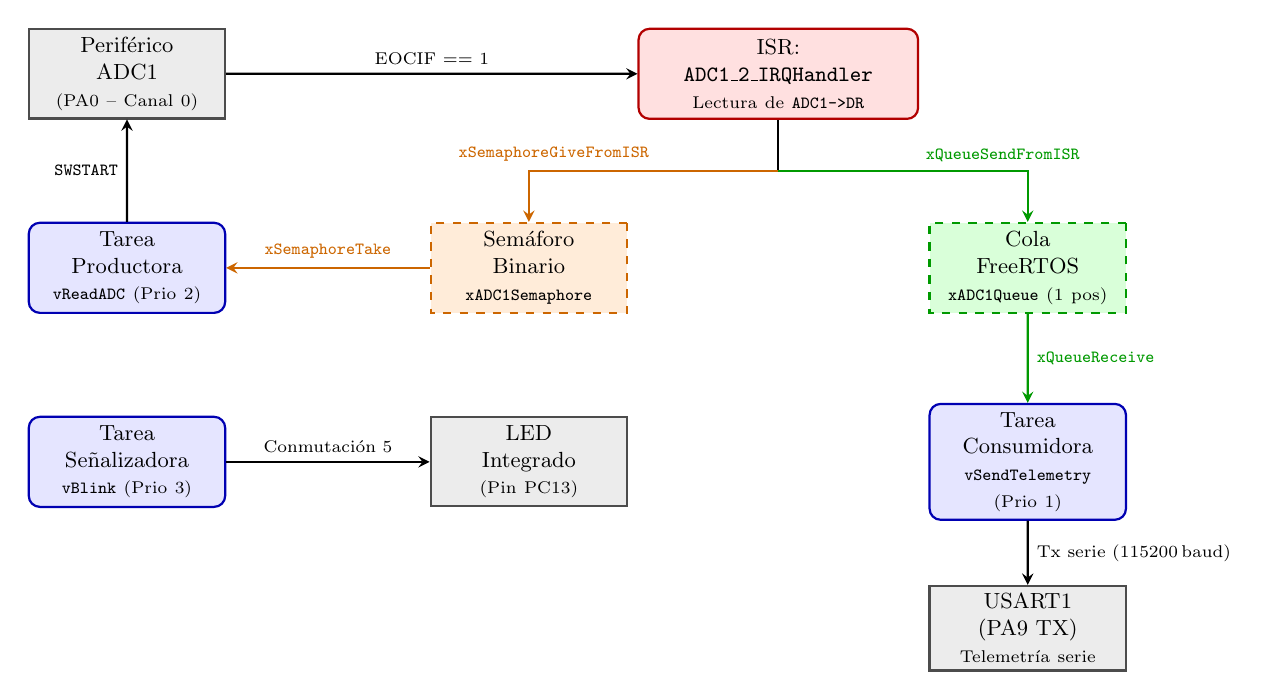
\begin{tikzpicture}[
    scale=0.88, transform shape,
    >=stealth,
    font=\small,
    block/.style={rectangle, draw=blue!70!black, thick, fill=blue!10, align=center, rounded corners=4pt, minimum height=1.3cm, text width=2.6cm},
    hw/.style={rectangle, draw=black!70, thick, fill=gray!15, align=center, minimum height=1.2cm, text width=2.6cm},
    isr/.style={rectangle, draw=red!70!black, thick, fill=red!12, align=center, rounded corners=4pt, minimum height=1.3cm, text width=3.8cm},
    queue/.style={rectangle, draw=green!60!black, thick, fill=green!15, dashed, align=center, minimum height=1.3cm, text width=2.6cm},
    sem/.style={rectangle, draw=orange!80!black, thick, fill=orange!15, dashed, align=center, minimum height=1.3cm, text width=2.6cm}
  ]

  % Fila 1: Periférico ADC e ISR (y = 4.2)
  \node[hw] (adc) at (0, 4.2) {Periférico\\ADC1\\{\scriptsize (PA0 -- Canal 0)}};
  \node[isr] (isr) at (9.4, 4.2) {ISR:\\\texttt{ADC1\_2\_IRQHandler}\\{\scriptsize Lectura de \texttt{ADC1->DR}}};

  % Fila 2: Tarea Productora y primitivas IPC (y = 1.4)
  \node[block] (task_prod) at (0, 1.4) {Tarea\\Productora\\{\scriptsize \texttt{vReadADC} (Prio 2)}};
  \node[sem] (sem) at (5.8, 1.4) {Semáforo\\Binario\\{\scriptsize \texttt{xADC1Semaphore}}};
  \node[queue] (queue) at (13.0, 1.4) {Cola\\FreeRTOS\\{\scriptsize \texttt{xADC1Queue} ($1$ pos)}};

  % Fila 3: Tarea Señalizadora, LED y Tarea Consumidora (y = -1.4)
  \node[block] (task_blink) at (0, -1.4) {Tarea\\Señalizadora\\{\scriptsize \texttt{vBlink} (Prio 3)}};
  \node[hw] (led) at (5.8, -1.4) {LED\\Integrado\\{\scriptsize (Pin PC13)}};
  \node[block] (task_cons) at (13.0, -1.4) {Tarea\\Consumidora\\{\scriptsize \texttt{vSendTelemetry} (Prio 1)}};

  % Fila 4: Periférico UART (y = -3.8)
  \node[hw] (uart) at (13.0, -3.8) {USART1\\(PA9 TX)\\{\scriptsize Telemetría serie}};

  % Punto de bifurcación desde la ISR
  \coordinate (fork) at (9.4, 2.8);

  % Conexión Productor -> ADC -> ISR
  \draw[->, thick] (task_prod) -- node[left, font=\scriptsize] {\texttt{SWSTART}} (adc);
  \draw[->, thick] (adc) -- node[above, font=\scriptsize] {EOCIF == 1} (isr);

  % Conexiones desde ISR hacia Semáforo y Cola
  \draw[thick] (isr.south) -- (fork);
  \draw[->, thick, orange!80!black] (fork) -| node[pos=0.45, above, font=\scriptsize] {\texttt{xSemaphoreGiveFromISR}} (sem.north);
  \draw[->, thick, green!60!black] (fork) -| node[pos=0.45, above, font=\scriptsize] {\texttt{xQueueSendFromISR}} (queue.north);

  % Sincronización del Productor mediante Semáforo
  \draw[->, thick, orange!80!black] (sem) -- node[above, font=\scriptsize] {\texttt{xSemaphoreTake}} (task_prod);

  % Flujo de la Cola hacia el Consumidor y Transmisión UART
  \draw[->, thick, green!60!black] (queue) -- node[right, font=\scriptsize] {\texttt{xQueueReceive}} (task_cons);
  \draw[->, thick] (task_cons) -- node[right, font=\scriptsize] {Tx serie ($115200\,\mathrm{baud}$)} (uart);

  % Señalización independiente
  \draw[->, thick] (task_blink) -- node[above, font=\scriptsize] {Conmutación $5\Hz$} (led);

\end{tikzpicture}

\caption{Diagrama de bloques y flujo de sincronización productor-consumidor en el Ejercicio 2.}
\label{fig.ej2:arquitectura}
\end{figure}

\section{Recursos de FreeRTOS Utilizados}
\label{sec.ej2:recursos}

Para resolver el desacoplamiento temporal y la transferencia segura de información entre los distintos contextos de
ejecución se recurrió a los siguientes componentes del kernel:

\subsection{Colas de Mensajes}

La comunicación entre el contexto de interrupción y la tarea consumidora se resuelve mediante una cola unidireccional
creada en el arranque del sistema:

\begin{lstlisting}[language=C]
xADC1Queue = xQueueCreate(1, sizeof(uint32_t));
\end{lstlisting}

La cola se dimensionó con una profundidad unitaria (\texttt{uxQueueLength = 1}) y un tamaño de elemento de cuatro bytes
(\texttt{sizeof(uint32\_t)}), suficiente para alojar la palabra de datos entregada por el convertidor de doce bits.

FreeRTOS implementa el pasaje de datos por copia, lo que asegura que el valor transferido
se preserve en el búfer interno administrado por el kernel, independientemente del ciclo de vida de las variables
locales de la rutina de interrupción.

Desde la rutina de servicio \texttt{ADC1\_2\_IRQHandler()}, el envío se efectúa mediante la variante especializada
para interrupciones:

\begin{lstlisting}[language=C]
BaseType_t xHigherPriorityTaskWoken = pdFALSE;
uint32_t ulADC1Value = ADC1->DR & ADC_DR_DATA_Msk;
xQueueSendFromISR(xADC1Queue, &ulADC1Value, &xHigherPriorityTaskWoken);
\end{lstlisting}

En la tarea consumidora, la extracción del elemento se lleva a cabo dentro de la función \texttt{vSendTelemetry()}:

\begin{lstlisting}[language=C]
uint32_t ulADC1Value;
xQueueReceive(xADC1Queue, &ulADC1Value, 0);
\end{lstlisting}

Al especificarse un tiempo de espera nulo (\texttt{xTicksToWait = 0}), la llamada no suspende a la tarea si la cola se
encuentra transitoriamente desprovista de nuevos elementos, procediendo a emitir la última lectura disponible.

\subsection{Semáforos Binarios}

La señalización del evento de fin de conversión se implementa a través de un semáforo binario creado con la función
\texttt{xSemaphoreCreateBinary()}:

\begin{lstlisting}[language=C]
xADC1Semaphore = xSemaphoreCreateBinary();
\end{lstlisting}

Al crearse, el semáforo binario se encuentra en estado vacío. Cuando el conversor analógico-digital completa el ciclo
de aproximaciones sucesivas, la rutina de interrupción cede el semáforo invocando:

\begin{lstlisting}[language=C]
xSemaphoreGiveFromISR(xADC1Semaphore, &xHigherPriorityTaskWoken);
\end{lstlisting}

En la tarea productora \texttt{vReadADC()}, la instrucción:

\begin{lstlisting}[language=C]
ADC1->CR2 |= ADC_CR2_SWSTART;
xSemaphoreTake(xADC1Semaphore, 0);
\end{lstlisting}

inicia la conversión y toma el testigo de sincronización generado por el periférico.

\subsection{Conmutación de Contexto con \textit{portYIELD\_FROM\_ISR}}

Un aspecto relevante de la interacción entre las interrupciones del microcontrolador y el planificador de FreeRTOS
reside en la macro \texttt{portYIELD\_FROM\_ISR()}:

\begin{lstlisting}[language=C]
void ADC1_2_IRQHandler(void) {
    BaseType_t xHigherPriorityTaskWoken;
    uint32_t ulADC1Value = ADC1->DR & ADC_DR_DATA_Msk;
    xQueueSendFromISR(xADC1Queue, &ulADC1Value, &xHigherPriorityTaskWoken);
    xSemaphoreGiveFromISR(xADC1Semaphore, &xHigherPriorityTaskWoken);
    portYIELD_FROM_ISR(xHigherPriorityTaskWoken);
}
\end{lstlisting}

Cuando una función con sufijo \texttt{FromISR} desbloquea una tarea cuya prioridad es superior a la de la tarea que
se encontraba en ejecución al dispararse la interrupción, la variable \texttt{xHigherPriorityTaskWoken} se establece
internamente en \texttt{pdTRUE}. Tan pronto como la rutina de interrupción retorna, el procesador
no regresa a la tarea que fue interrumpida, sino que conmuta directamente el contexto hacia la tarea de mayor prioridad
recién desbloqueada, minimizando la latencia de respuesta del sistema. Esto es posible gracias a una interrupcion por
software.

  \chapter{Conclusiones}

El desarrollo del presente trabajo práctico permitió implementar y validar de forma experimental los conceptos
centrales del diseño de aplicaciones embebidas basadas en FreeRTOS sobre la arquitectura ARM Cortex-M3. A través
de los ejercicios planteados se superó la estructura tradicional de super-loop, sustituyéndola por una arquitectura
modular dividida en tareas con prioridades bien definidas, colas de mensajes y semáforos de sincronización.


  
  \nocite{*}
  \printbibliography[heading=bibnumbered, title={Fuentes}]
  
  \chapter{Anexos}
\label{sec.anexos:codigo}

\section{Código Fuente del Ejercicio Práctico N.º 1}

A continuación se presenta el código completo del archivo \texttt{main.c} correspondiente al Ejercicio 1,
donde se implementan las tareas de señalización luminosa y telemetría junto al gancho de inactividad.

\lstinputlisting[
  language=C,
  caption={Código fuente completo de \texttt{main.c} para el Ejercicio 1.},
  label={list.ej1:main}
]{sources/ep1/src/main.c}

\newpage

\section{Código Fuente del Ejercicio Práctico N.º 2}

A continuación se transcribe el código del archivo \texttt{main.c} correspondiente al Ejercicio 2,
incorporando el periférico ADC1, la rutina de interrupción \texttt{ADC1\_2\_IRQHandler}, la cola \texttt{xADC1Queue}
y el semáforo binario \texttt{xADC1Semaphore}.

\lstinputlisting[
  language=C,
  caption={Código fuente completo de \texttt{main.c} para el Ejercicio 2.},
  label={list.ej2:main}
]{sources/ep2/src/main.c}

\newpage

\section{Configuración del Kernel (\texttt{FreeRTOSConfig.h})}

En este anexo se adjunta el archivo de cabecera \texttt{FreeRTOSConfig.h} empleado para parametrizar el núcleo del
sistema operativo en ambos ejercicios prácticos.

\lstinputlisting[
  language=C,
  caption={Archivo de configuración \texttt{FreeRTOSConfig.h} del kernel para STM32F103.},
  label={list.config:freertos}
]{sources/ep1/include/FreeRTOSConfig.h}

\end{document}
